\documentclass[10pt]{article}
\usepackage{icmlko}

\icmlmeta{IP 파운데이션 월드모델}{147}{한계는 숫자가 아니라 행렬이었다}{노트 146이 순위표에 띠 하나를 얹고 ``위 여섯은 순위가 없다''고 했다. 띠가 짝마다 여섯 배 다르고, 제대로 재니 없다던 순위 하나가 돌아온다}

\begin{document}

\twocolumn[
\icmlheader

\begin{abstract}
노트 146이 판 $\rho$의 씨앗 표준편차 0.0087을 순위표 전체에 얹고 ``상위
격차 열둘 중 열이 그 아래 --- 위 여섯은 순위가 없다''고 적었다. \textbf{잣대가
틀렸다.} 두 정식화를 견줄 때 표본 잡음은 \emph{같은 레코드}에 걸리므로
차에서 대부분 상쇄된다. 순위를 가르는 값은 주변 sd 가 아니라 \textbf{짝
sd} 이고, 그것은 두 정식화가 얼마나 닮았느냐에 따라 달라진다. 쟀다 ---
\textbf{주변 sd 는 일곱 정식화 전부 0.016$\sim$0.018로 사실상 같은데 짝 sd 는
0.0027에서 0.0174까지 6.4배 벌어진다.} 닮은 짝(F6 능형 대 F9 순위우도, 둘
다 같은 자질의 선형)은 0.0027이고 안 닮은 짝(F8 부스팅 대 F7 닻)은 0.0174다.
\textbf{그러니 판에 ``탐지 한계'' 숫자 하나를 붙이는 것은 두 방향으로
틀린다} --- 닮은 짝에는 너무 엄하고 안 닮은 짝에는 너무 무르다. 한계는
행렬이다. 그 행렬로 일곱 정식화를 다시 세우니 \textbf{네 칸의 부분 순서}가
나온다: \{F18 배깅, F8 부스팅\} $>$ F10 도메인수축 $>$ \{F12, F6, F9\} $>$
F7 닻. \textbf{주변 잣대로는 F10 이 셋째 칸에 묻힌다} --- 격차가
0.018$\sim$0.022로 주변 문턱 0.036에 못 미친다. 짝 sd 는 0.0069$\sim$0.0074라
$t=2.5\sim2.9$로 갈린다. \textbf{잣대를 고치니 없던 순위 한 칸이 돌아왔다.}
반대로 1칸의 F18 대 F8은 여전히 안 갈린다 --- 격차 $+$0.0050에 짝 sd
0.0062($t=0.8$)이고, 그 sd 의 절반 이상이 씨앗 잔여항이다. 예측을 씨앗
셋으로 평균해도 씨앗 분산은 $\sqrt{3}$으로 줄 뿐이다.
\end{abstract}
]

\begin{figure*}[t]
\centering
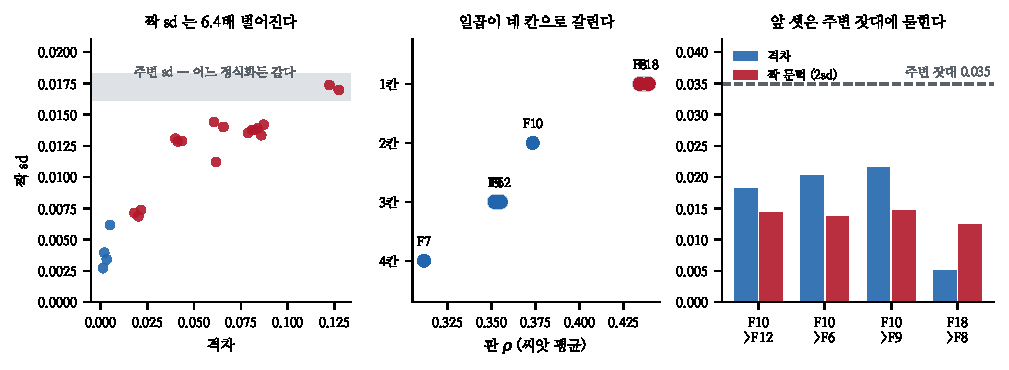
\includegraphics[width=\textwidth]{figs/order.pdf}
\caption{왼쪽 --- 주변 sd 는 다 같고 짝 sd 는 6.4배 벌어진다. 가운데 ---
일곱이 네 칸으로 갈린다. 오른쪽 --- 앞 셋은 주변 잣대에 묻힌다.}
\end{figure*}

\section{잣대가 짝마다 다르다}

\claimx{\textbf{표본 잡음은 짝에서 상쇄된다.} 두 정식화를 같은 재추출로
채점하면 ``이번 표본이 쉬웠다''가 양쪽에 똑같이 걸린다. 남는 것은 두
정식화가 \emph{다르게 매긴} 부분뿐이다.}{그러니 짝 sd 는 두 예측의 상관에
달렸다. 상관이 1이면 0, 무관이면 주변 sd 의 $\sqrt2$배다.}

\begin{table}[t]
\centering\tsize
\caption{판 $\rho$의 흔들림. 문턱 40 · 검색$+$달력 · 재추출 400.}
\begin{tabular}{lr}
\toprule
주변 sd (일곱 정식화) & .0161 $\sim$ .0183 \\
\midrule
짝 sd --- F6 대 F9 & \textbf{.0027} \\
짝 sd --- F12 대 F9 & .0034 \\
짝 sd --- F10 대 F6 & .0069 \\
짝 sd --- F18 대 F10 & .0140 \\
짝 sd --- F8 대 F7 & \textbf{.0174} \\
\bottomrule
\end{tabular}
\end{table}

\claimx{\textbf{주변은 같고 짝은 6.4배 벌어진다.} 주변 sd 로는 일곱이
구별이 안 되는데 --- 다 0.017 언저리다 --- 짝 sd 는 어느 둘을 견주느냐에
따라 0.0027에서 0.0174까지 간다.}{짝 sd 에는 표본 항 말고 \emph{씨앗
잔여항}도 있다. 예측을 씨앗 셋으로 평균해도 씨앗 분산은 $\sqrt3$으로 줄
뿐이라, F18 대 F8 에서는 그 항이 0.0050으로 표본 항 0.0036보다 크다.}

\section{네 칸의 부분 순서}

\begin{table}[t]
\centering\tsize
\caption{일곱 정식화. 예측을 씨앗 셋으로 평균한 뒤.}
\begin{tabular}{llr}
\toprule
칸 & 정식화 & 판 $\rho$ \\
\midrule
\textbf{1} & F18 배깅 & \textbf{$+$.4391} \\
& F8 부스팅 & $+$.4341 \\
\textbf{2} & F10 도메인수축 & $+$.3735 \\
\textbf{3} & F12 순위합집합 & $+$.3553 \\
& F6 직접풀링 & $+$.3532 \\
& F9 순위우도 & $+$.3519 \\
\textbf{4} & F7 닻 & $+$.3119 \\
\bottomrule
\end{tabular}
\end{table}

\claimx{\textbf{일곱이 네 칸으로 갈린다.} 스물한 짝 중 열일곱이 갈리고
넷이 안 갈린다. 노트 146의 ``위 여섯은 순위가 없다''는 과장이었다 ---
없는 것은 칸 \emph{안}의 순위지 칸 사이가 아니다.}{칸 나누기는 문턱
$2\,\mathrm{sd}$의 함수다. $3\,\mathrm{sd}$로 올리면 F10 이 셋째 칸으로
내려가 세 칸이 된다.}

\section{잣대를 고치니 한 칸이 돌아왔다}

\begin{table}[t]
\centering\tsize
\caption{주변 잣대(2$\times$0.017 = 0.035)로는 묻히는 짝.}
\begin{tabular}{lrrr}
\toprule
& 격차 & 짝 sd & $t$ \\
\midrule
F10 $>$ F9 & $+$.0216 & .0074 & \textbf{2.9} \\
F10 $>$ F6 & $+$.0202 & .0069 & \textbf{2.9} \\
F10 $>$ F12 & $+$.0182 & .0071 & \textbf{2.5} \\
\midrule
F18 $>$ F8 & $+$.0050 & .0062 & 0.8 \\
\bottomrule
\end{tabular}
\end{table}

\claimx{\textbf{F10 도메인수축이 선형 셋을 진짜로 이긴다.} 격차가
0.018$\sim$0.022로 주변 문턱 0.035에 한참 못 미치는데, 짝 sd 가
0.0069$\sim$0.0074라 $t=2.5\sim2.9$다. 주변 잣대를 쓰면 이 셋이 한 칸에
뭉쳐 \emph{보이지 않는 결론}이 된다.}{F10 은 노트 132에서 만든 도메인별
수축이다. 그때는 판이 $+$0.3735로 F8($+$0.4328)에 밀려 접었는데, 선형
계열은 이긴다는 것이 이제 보인다.}

\claimx{\textbf{반대로 1칸은 여전히 안 갈린다.} F18 대 F8 은 $+$0.0050에
짝 sd 0.0062다. 노트 145 · 146이 세 번 다르게 재고 세 번 다 ``안 갈린다''를
얻었는데, 네 번째로 제대로 재도 같다.}{그 sd 의 0.0050이 씨앗 잔여항이다
--- 표본을 늘려도 안 줄고 씨앗을 늘려야 준다. 씨앗 아홉이면 0.0029로
내려가 $t=1.3$이 된다. 그래도 안 갈린다.}

\section{판정 도구로 넣었다}

\texttt{lab/rank.py} 에 넣었다. \texttt{predictions()} 는 씨앗을 갈아
끼워 적합하고 예측 \emph{순위}를 평균한다(점수가 아니라 예측을 평균해야
분산이 실제로 준다). \texttt{resolve()} 는 같은 재추출을 모든 정식화에
써서 짝 sd 를 내고 부분 순서를 짠다.

\begin{table}[t]
\centering\tsize
\caption{이 판의 한계 셋. 셋 다 실행마다 적는다.}
\begin{tabular}{lll}
\toprule
& 재는 것 & 노트 \\
\midrule
분해능 & 표본이 작아 못 보는 차이 & 135 \\
귀착 & 풀이 흔들려 못 돌리는 차이 & 144 \\
\textbf{짝 분해능} & \textbf{두 정식화를 가르는 데 드는 차이} & \textbf{147} \\
\bottomrule
\end{tabular}
\end{table}

\begin{table}[t]
\centering\tsize
\caption{남은 것.}
\begin{tabular}{ll}
\toprule
F10 & 선형을 이긴다 --- 부스팅과 섞으면 \\
1칸 & F18 대 F8 은 씨앗을 늘려도 안 갈린다 \\
축 세트 & 정식화가 아니라 축을 견줄 때도 짝이 맞나 \\
\bottomrule
\end{tabular}
\end{table}

첫 줄이 다음 자리다. F10 은 도메인마다 수축을 다르게 주는 선형이고 F8은
풀링 부스팅이다. 둘의 예측 상관이 낮다면(짝 sd 0.0140이 그렇다고 말한다)
섞을 자리가 있다 --- 노트 132에서 F10 을 접은 이유가 ``F8 보다 낮아서''
였는데, 낮은 것과 겹치는 것은 다르다.

\end{document}
